\chapter{Simulator}
\label{chap:sim}

\begin{figure}
	\centering
	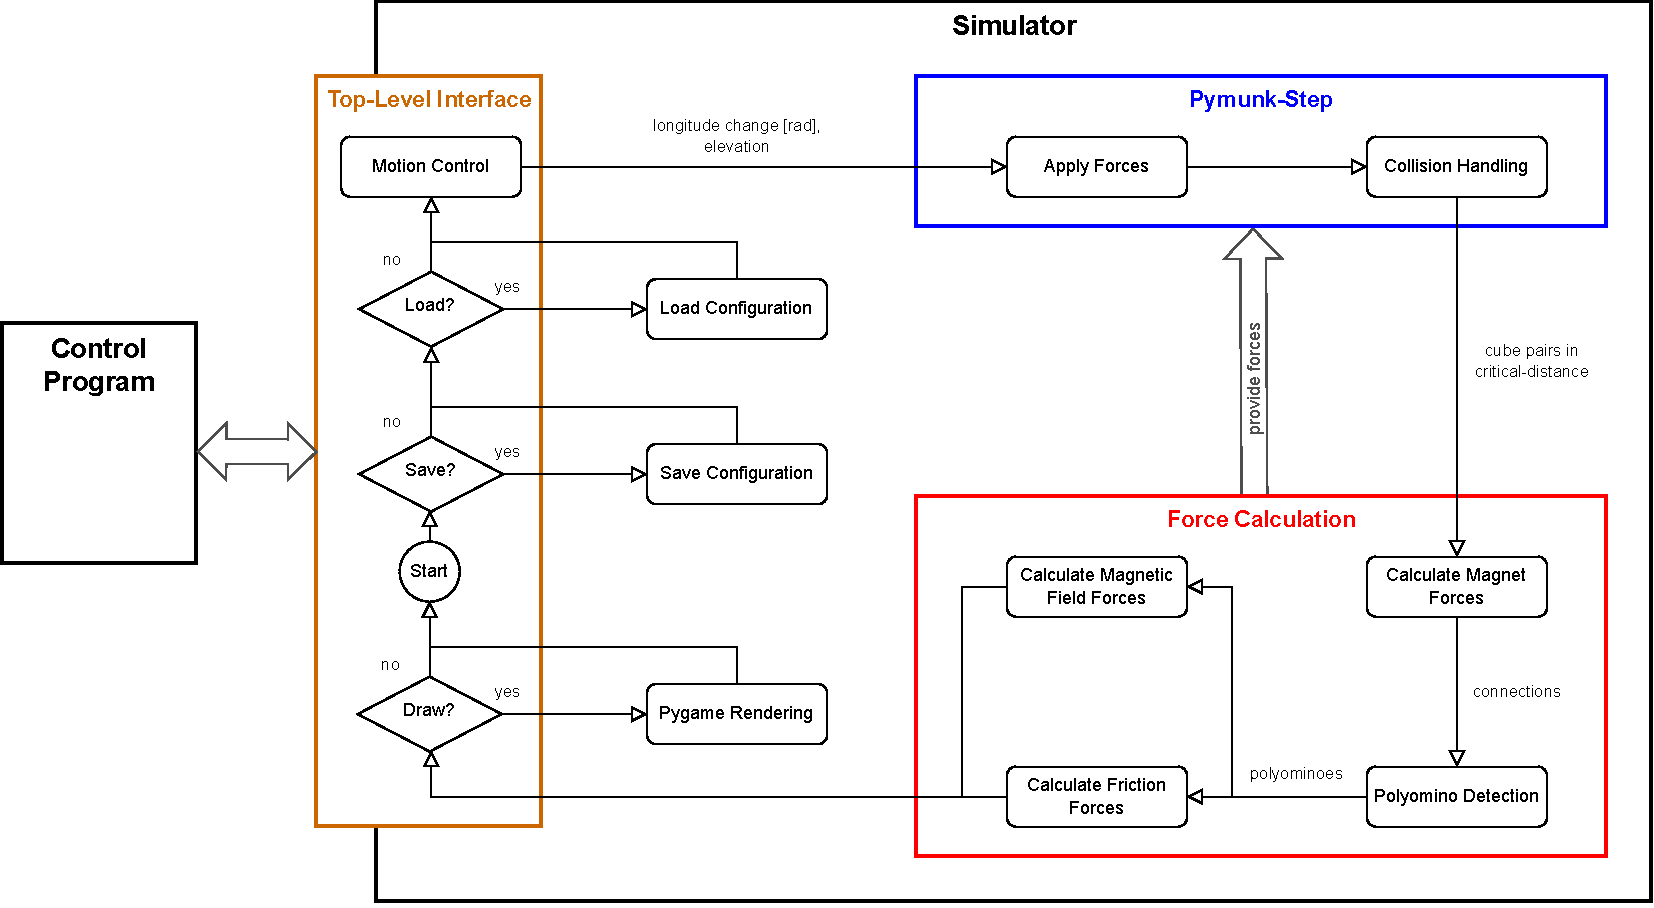
\includegraphics[width=1\textwidth]{figures/simulator_controlflow.pdf}
	\caption[Control flow of the simulator]{long caption...}
	\label{fig:simulator}
\end{figure}

Our simulator used for modeling the behavior of magnetic modular cubes uses the 2d physics library Pymunk\footnote{Pymunk: \url{https://www.pymunk.org/}}.
This library is build for the Python 3 and Python 2 environment based on the 2d physics library Chipmunk\footnote{Chipmunk: \url{http://chipmunk-physics.net/}}.
We used Pymunk, since it can be easily integrated and customized in a Python implementation.
Furthermore it is light-weight and capable of running headless, but also offers an interface for Pygame\footnote{Pygame: \url{https://www.pygame.org/}}, which we use to visualize developed plans and allow user control.
As a disadvantage, we are challenge with the simulation of 3d movement in a 2d environment.
That way we trade simulation accuracy for faster simulation time, which is necessary to develop global plans in reasonable time.

\autoref{fig:simulator} shows a flow chart diagram of the simulators simulation loop.
The diagram provides the control flow of our simulator, where individual steps are explained in this and following sections.

Any control program, in example a local planner or a ``sandbox mode'' for visually controlling magnetic modular cubes with keyboard inputs, can interact with the top-level interface of the simulator.
The interface provides functionalities like, starting and stopping the simulation process, loading custom configurations and retrieving the current workspace state (\autoref{sec:motion_control}), queuing in motions for simulation (\autoref{sec:workspace_state}), or controlling the drawing with Pygame.
The Pymunk-Step is a library function, responsible for updating the Pymunk-Space by a certain time step.
The duration of a time step is a parameter that also allows the adjustment between simulation accuracy and simulation time.
Inside the Pymunk-Step forces are applied to the cubes and collision with workspace boundaries and between cubes is handled.
%force calculation
%friction for 3d 

% plot of time use for simulation


\section{Motion Control}
\label{sec:motion_control}

% rotaion linear ramp
% step sequence for motions
% handling elevation in 2D with friction
% waiting on motions to finish

\section{Workspace State}
\label{sec:workspace_state}

% what configuration consists of.
% cube info, poly info.
% polycollection functions as set and lists for polys
% everything hashable
% loading saving configs 

\section{Collision Handling}

% pymunks colison detection for cubes and walls -> Bounding volume hirachie
% used to determine range for magnetic forces

\section{Simulating Forces}

% apply with pymunk

\subsection{Magnet Forces}

% pull cubes together
% provide equation
% plot for magnetic attraction based on distance
% hold cubes together -> polyomino detection
% wich magnetic pairs to choose
% minDist, minDists, all

\subsection{Magnetic Field Forces}

% applied to top bottom each indivial cube
% as long as orientation doenst match
% the bigger the poly the longer rotations actually take 
% adding zero updates to motion so that motion finishes when polys oriented


\subsection{Friction Forces}

% force to let poly rotate around pivot point
% splitt friction on cubes on pivot edge
% nominal friction to prevent breaking


